\documentclass[runningheads,a4paper]{llncs}
% proper encoding
\usepackage[T1]{fontenc}

% autoref command
\usepackage[pdftex,urlcolor=black,colorlinks=true,linkcolor=black,citecolor=black]{hyperref}

% better typography
\usepackage[activate=compatibility]{microtype}

% graphics
\usepackage{graphicx}

\usepackage[lofdepth,lotdepth]{subfig}

% URLs
\usepackage{url}

\begin{document}

\mainmatter

\title{Enriching Content Objects for Multimodal Search with Data from the Linking Open Data Cloud}
\authorrunning{Enriching Content Objects for Multimodal Search with Data from the Linking Open Data Cloud}

\author{Jonas Etzold\inst{1} \and Thomas Steiner\inst{2} \and Arnaud Brousseau\inst{2}\thanks{The author was an intern at Google Germany GmbH at time of core development.} \and Paul Grimm\inst{1}}

\institute{\label{fulda}Hochschule Fulda, Marquardstr. 35
36039 Fulda, Germany\\
\urldef{\emails}\path|{jonas.etzold,paul.grimm}@hs-fulda.de|\emails\\
\and Google Germany GmbH, ABC-Str. 19, 20355 Hamburg, Germany\\
\urldef{\emails}\path|{tomac,arnaudb}@google.com|\emails\\
}

\maketitle

\begin{abstract}
In this paper, we report on work around the \mbox{I-SEARCH} EU (FP7 ICT STREP) project
whose objective is the development of a multimodal search engine that supports multimodal
in- and output, as well as multimodal  query refinement.
Supported modalities and combinations thereof are \emph{audio}, \emph{video},
\emph{rhythm}, \emph{image}, \emph{3D object}, \emph{sketch}, \emph{emotion},
\emph{social signals}, \emph{geolocation}, and \emph{text}.
An important aspect for \mbox{I-SEARCH} to work is the so-called
\emph{Rich Unified Content Description} \emph{\mbox{(RUCoD)}} format
consisting of a multi-layered structure
for the description of low and high level features of content objects.
The \emph{\mbox{(RUCoD)}} description format allows content objects
to be queried in a consistent way by using extracted \mbox{\emph{RUCoD}} features.
During the session, we will present a live demonstration of the \mbox{I-SEARCH}
Graphical User Interface (GUI) prototype and, via pre-defined use cases,
show how we imagine multimodal search in the future.
We are especially looking for networking opportunities with projects dealing with
semantic annotation of large-scale multimedia content pools and 
projects interested in our \emph{RUCoD} feature extraction techniques.
\end{abstract}

\section{Introduction}

\section{Rich Unified Content Description (RUCoD)}
It is evident that for the outlined scenarios to work, a significant investment in describing the underlying media items is necessary.
Therefore, in~\cite{ijmis2010}, we have first introduced the concept of so-called \emph{content objects}, and second, a description format named \emph{Rich Unified Content Description \mbox{(RUCoD)}}.
Content objects are rich media presentations, enclosing different types of media, along with real-world information and user-related information.
\mbox{\emph{RUCoD}} provides a uniform descriptor for all types of content objects, irrespective of the underlying media and accompanying information.
Due to the enormous processing costs for the description of content objects,
our approach currently is not yet applicable on Web scale.
We target ``Company Wide Intraweb'' scale rather than World Wide Web scale environments,
which, however, we make accessible in a multimodal way from the World Wide Web.

\begin{figure}[]
  \centering
    \subfloat[][Architecture of the CoFetch tool.]{
      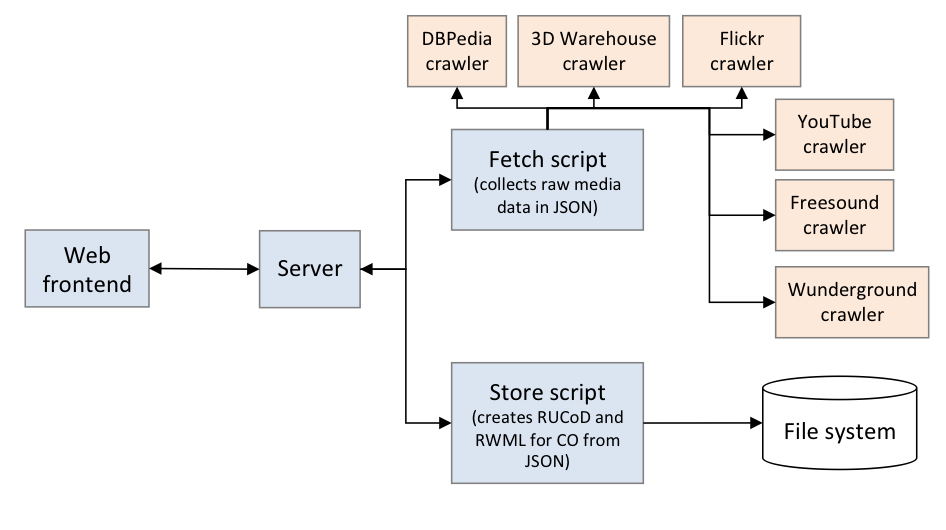
\includegraphics[width=0.5\textwidth]{architecture.png}
      \label{fig:architecture}}
    \qquad
    \subfloat[][Screenshot of the CoFetch tool.]{
      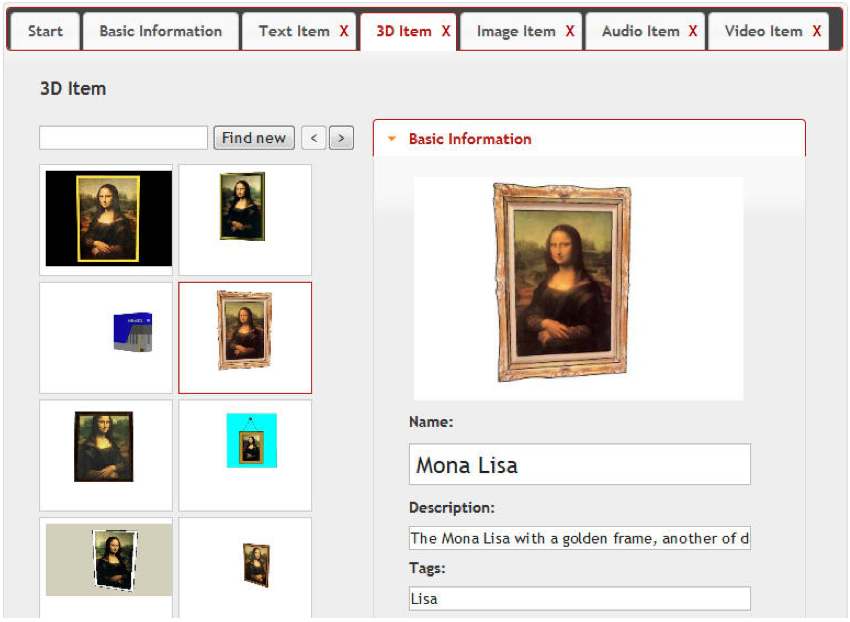
\includegraphics[width=0.4\textwidth]{screenshot.png}
      \label{fig:screenshot}}
\caption{CoFetch.}
\label{fig:cofetch}
\end{figure}

\bibliographystyle{splncs03}
\bibliography{eswc2012}

\end{document}